\section{Energieverlust von $\alpha$-Strahlung in Luft}
%kurz das ziel dieses versuchsteiles ansprechen, damit keine zwei �berschriften direkt �bereinander stehen!
%bei schwierigeren versuchen kann auch der theoretische hintergrund erl�utert werden. (mit formeln, herleitungen und erkl�rungen)
In diesem Versuchsabschnitt soll der Energieverlust von $\alpha$-Strahlung in Luft, bei Normaldruck untersucht werden.

\subsection{Versuchsdurchf�hrung}
Da wie zuvor der Abstand zwischen dem Pr�parat und dem Detektor nicht variierbar ist, wird der Druck variiert. Die Spektroskopiekammer wird evakuiert. Dann werden der Verst�rker und der ACD so eingestellt, so dass das $^{226}$Ra-Spektrum deutlich zu erkennen ist. Da im Bereich von niedrigen Energien ein starker Untergrund vorhanden ist muss die Einstellschraube LLD am ADC so eingestellt werde, dass der Untergrund m�glichst gut raus gefiltert wird. Dann wird eine Kanal-Zeit-Eichung mit der Zerfallsreihe von $^{266}$Ra durchgef�hrt. Die Zerfallsreihe ist in Abb. ?? zu sehen.

\begin{figure}[H]
	\centering
  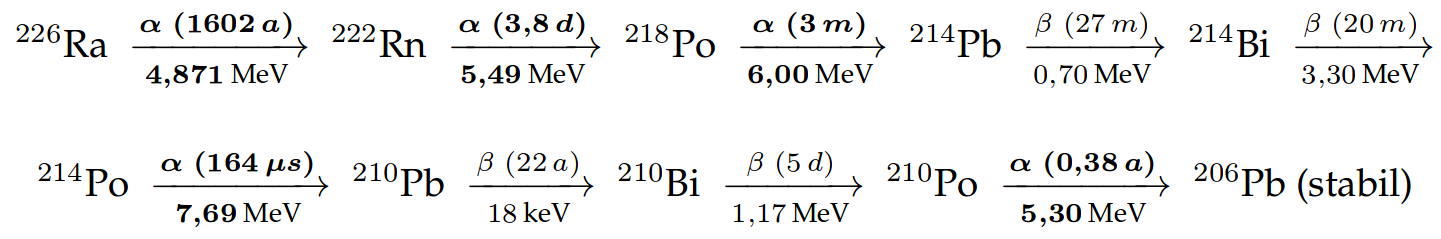
\includegraphics[scale=0.33]{zerfalls_reihe.png}
	\caption{Zerfallsreihe von $^{266}$Ra, entnommen von ??}
	\label{fig:kammer}
\end{figure}

Die Kammer wird langsam bel�ftet und Spektren im Bereich von 100 Torr bis 800 Torr in 25 Torr Schritten aufgenommen, wobei der Druck w�hrend der Messung konstant gehalten wird. Ein Bar entspricht 750.061683 Torr. Nach Gl. \ref{eqn:reich_normal} kann die Strecke mit erh�htem Druck in die Strecke unter Normaldruck umgerechnet werden. Aus den Countrates in Abh�ngigkeit des Drucks kann der absolute Energieverlust und der Energieverlust pro Wegst�ck bei Normaldruck bestimmt werden. F�r den Energieverlust pro Wegst�ck wird ein Verhalten nach Gl. ?? erwartet. Die Peaks der Spektren werden mit der Voigt-Verteilung gefittet.

\subsection{Auswertung}
In Abb. ?? sind die Messdaten mit dem Fit der Rutherfordstreuformel zu sehen. Die Rutherfordstreuuformel wurde nach GL. ?? gefittet. Dabei ergaben sich f�r den Fit die Werte in Tabelle ??.
